\documentclass[12pt,a4paper]{article}
\usepackage[T1]{fontenc}
\usepackage[utf8x]{inputenc}
\usepackage[french]{babel}
\usepackage{lmodern}
\usepackage{graphicx}
\usepackage{xcolor}
\usepackage{listings}
\usepackage{listingsutf8}
\usepackage{libertine}
\usepackage{microtype}
\usepackage{hyperref}

\title{Conception d'une application web de réservation\\[3mm] \normalsize{\it Laboratoire de technologie web}}
\author{Christophe Simon \\ Guillaume de Moffarts}
\date{\today}
\setlength\topmargin{-10mm}
\setlength\headheight{0mm}
\setlength\textheight{24cm}
\setlength\oddsidemargin{-0.5cm}
\setlength\textwidth{16.5cm}
\setlength{\parskip}{3mm}
\setlength{\parindent}{0mm}
%\usepackage{xcolor}

\lstdefinelanguage{CSS}
{morekeywords=[1]{color,border,text,decoration,margin,padding,left,top,right,background,font,size,weight,float, width, height, isplay, position, cursor, bottom, opacity, radius, content, family, transition, webkit, transform, max, overflow},
morekeywords=[2]{first,child,nth,of,type,letter,selection},
morekeywords=[3]{h1,p,div,tr,td},
morekeywords=[4]{},
morekeywords=[5]{},
sensitive,
morecomment=[s]{/*}{*/},}

\lstdefinelanguage{php}
{morekeywords=[1]{class,function,private,return,if,else,for,throw,new,null,while,for,foreach,as},
morekeywords=[2]{},
morekeywords=[3]{echo,Exception,exit,empty,header,isset,serialize,unserialize,count,array_push,array,die,sprintf, include},
morekeywords=[4]{\$this,\$_POST,\$_SESSION},
morekeywords=[5]{mysqli_query,mysqli_num_rows,mysqli_fetch_assoc,mysqli_connect,mysqli_close,mysqli_stmt_init,mysqli_stmt_prepare,mysqli_stmt_bind_param,mysqli_stmt_execute,mysqli_insert_id,mysqli_error,mysqli_connect_error},
morestring=[b]{"},
morestring=[b]{'},
morecomment=[l]{//},}

\lstset{
    extendedchars=\true,
    inputencoding=utf8x,
    basicstyle=\fontfamily{pcr}\selectfont\scriptsize\color{black},
    keywordstyle=[1]\color{blue}\bfseries, % style for keywords
    keywordstyle=[3]\color[rgb]{0,0.6,0}\bfseries, % style for keywords
    keywordstyle=[4]\color[rgb]{0.6,0,0}\bfseries, % style for keywords
    keywordstyle=[5]\color[rgb]{0,0.2,0}\bfseries, % style for keywords
    stringstyle=\color[rgb]{0.6,0.47,1}, %style between " "
    commentstyle=\color[rgb]{0.3,0.7,0.3},
    %numbers=left, % where to put the line-numbers
    %numberstyle=\tiny, % the size of the fonts that are used for the line-numbers
    showspaces=false, % show spaces adding particular underscores
    showstringspaces=false, % underline spaces within strings
    showtabs=false, % show tabs within strings adding particular underscores
    frame=single, % adds a frame around the code
    tabsize=2, % sets default tabsize to 2 spaces
    rulecolor=\color{black},
    captionpos=b, % sets the caption-position to bottom
    breaklines=true, % sets automatic line breaking
    breakatwhitespace=false,
    frame={}
}

\urlstyle{sf}
\newcommand{\file}[1]{"../#1"}

\begin{document}
	\maketitle
	\section*{Introduction}
		Dans le cadre du laboratoire de Technologie web, nous avons réalisé une application web dont le but est de réserver des billets d'avion. Le code de cette application suit le design pattern MVC (Model View Controller).

		Nous avons choisi comme idée de réaliser une caricature de la compagnie aérienne Ryanair, que nous avons appelée BryanAir. Le style de notre application a été inspiré du site officiel de la compagnie.

		Dans ce rapport se trouve une description du site et des explications sur le fonctionnement normal et erroné de l'application, ainsi qu'un diagramme de séquence pour illustrer cela.


	\section{Description du site}
		Il y a tout d'abord une page d'accueil menant vers la réservation (figure~\ref{fig:home}).
		\begin{figure}[!p]
			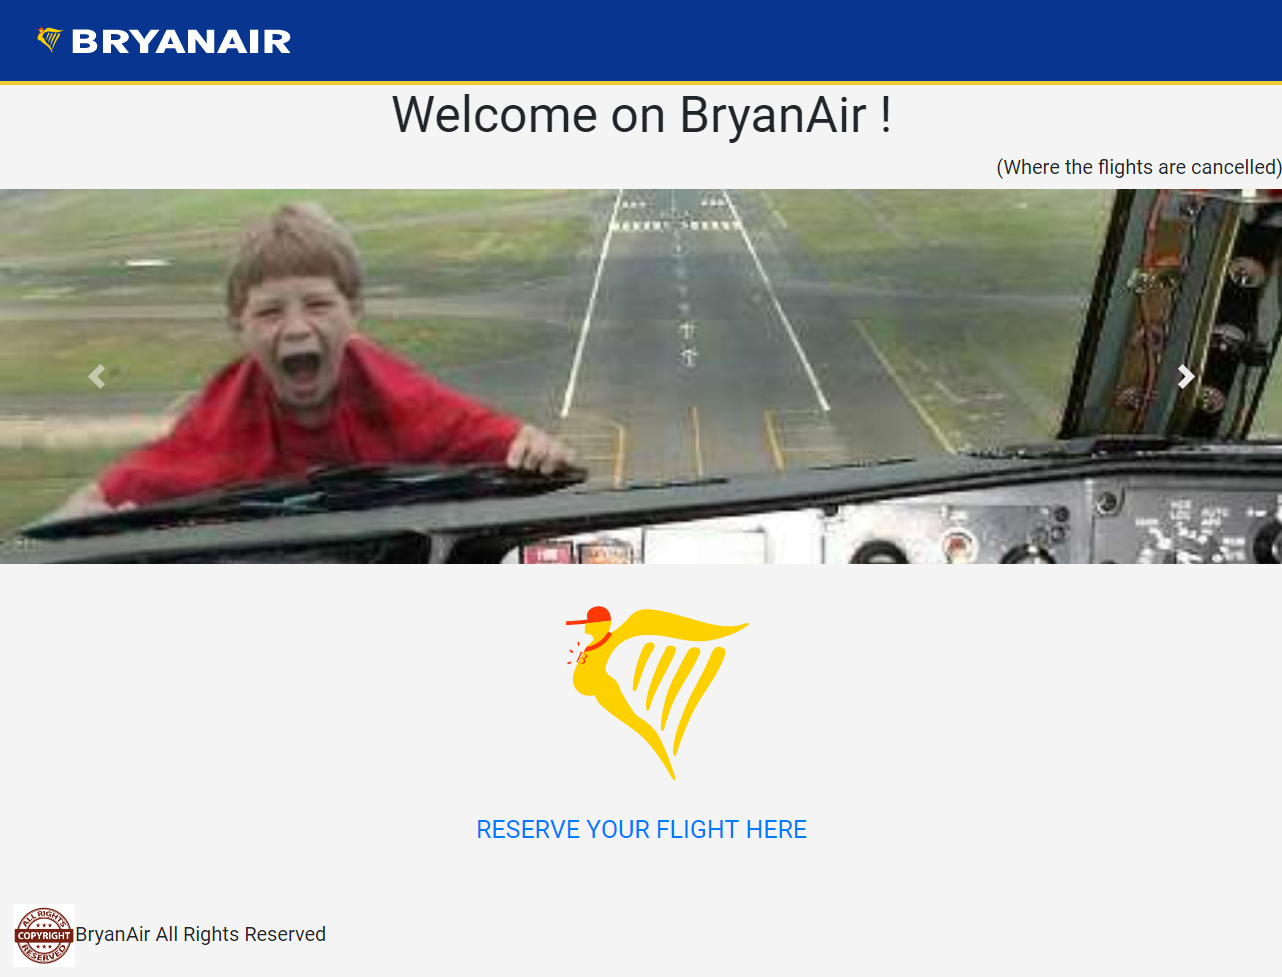
\includegraphics[width=\textwidth]{home.png}
			\caption{Page d'accueil.}
			\label{fig:home}
		\end{figure}

		La première page de réservation permet de réserver des billets pour un vol pour plusieurs passagers (figure~\ref{fig:res1}). Il faut préciser les aéroports de départ et d'arrivée, si on veut un aller simple ou un aller-retour, le nombre de passager(s), une adresse e-mail et si on désire une assurance annulation ou pas.
    La deuxième étape permet d'enregistrer les informations de chaque passager (nom, prénom et age) (figure~\ref{fig:res2}).
		\begin{figure}[!p]
      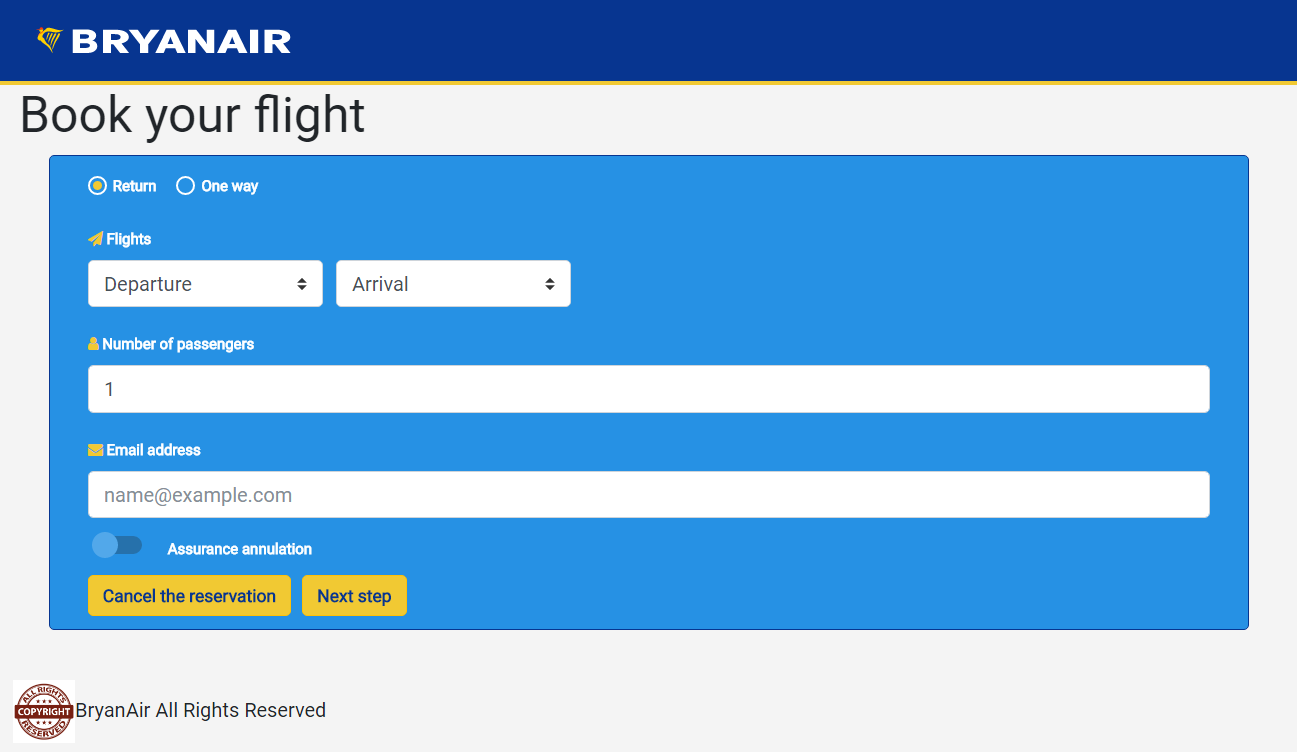
\includegraphics[width=\textwidth]{Reservation.png}
			\caption{Réservation étape 1.}
			\label{fig:res1}
		\end{figure}

		\begin{figure}[!p]
      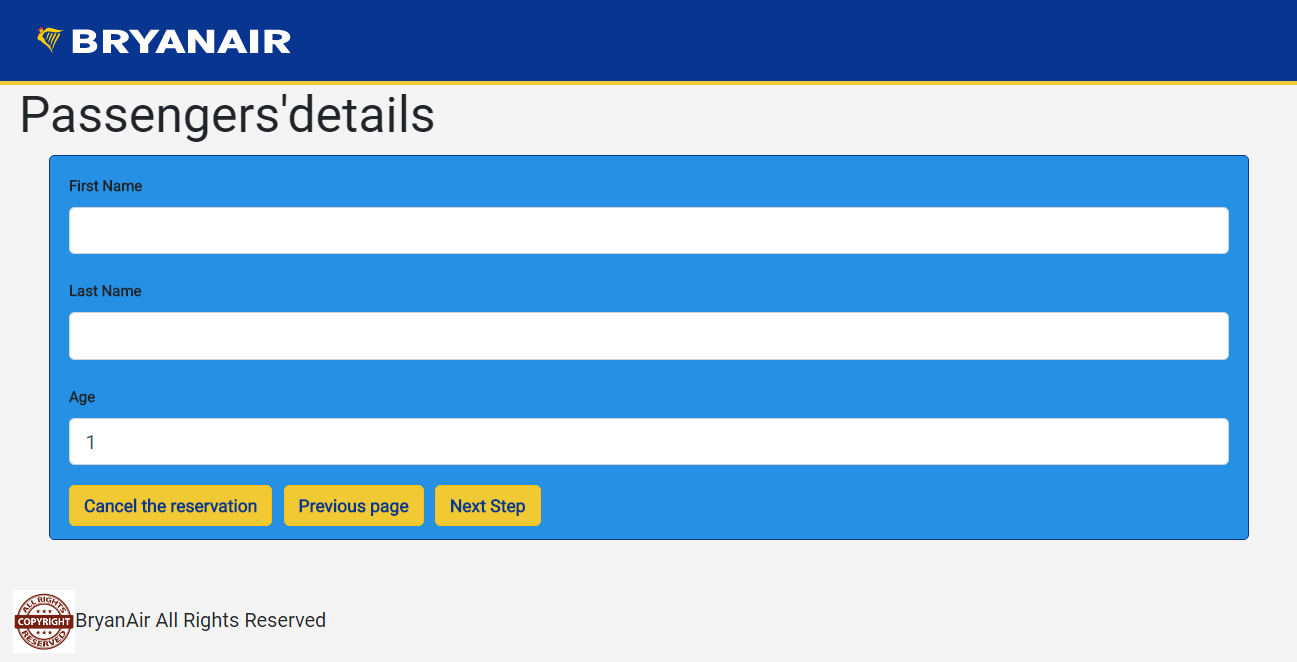
\includegraphics[width=\textwidth]{Detail.png}
			\caption{Réservation étape 2.}
			\label{fig:res2}
		\end{figure}

		Une fois tous les passagers enregistrés, on arrive sur une page de confirmation où vous avez le choix de confirmer ou d'annuler votre réservation (figure~\ref{fig:conf}).Une fois celle-ci confirmée, on arrive sur une page récapitulative de la commande avec le prix total à payer (figure~\ref{fig:recap}).

		\begin{figure}[!p]
      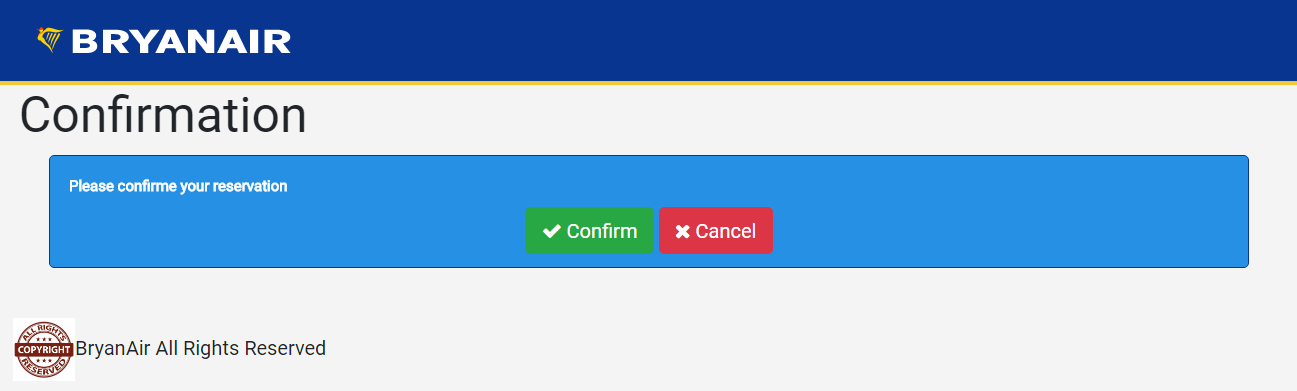
\includegraphics[width=\textwidth]{Confirmation.png}
			\caption{Confirmation.}
			\label{fig:conf}
		\end{figure}

		\begin{figure}[!p]
      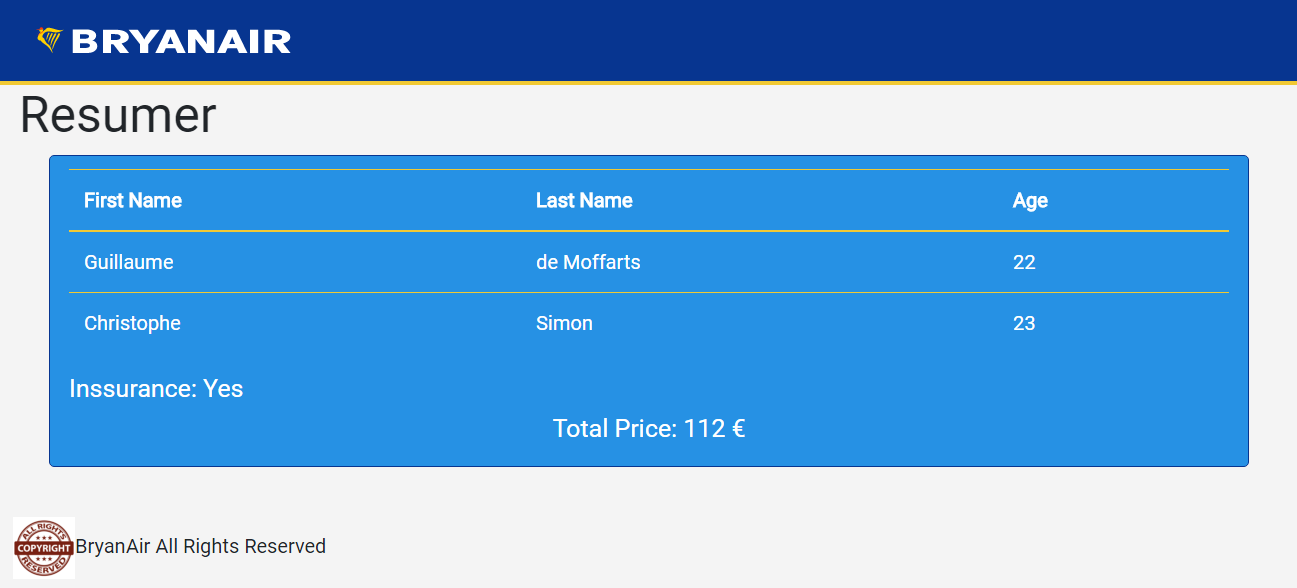
\includegraphics[width=\textwidth]{Resumer.png}
			\caption{Récapitulatif.}
			\label{fig:recap}
		\end{figure}

		Enfin, il y a une page d'administration où l'on peut voir, éditer ou supprimer les passagers pour chaque vol (figure~\ref{fig:admin}). Cette page ne devant pas être accessible au public, il n'y a pas de bouton pour y accéder. L'accès se fait directement par \url{http://localhost/BryanAir/admin}.

		\begin{figure}[!p]
      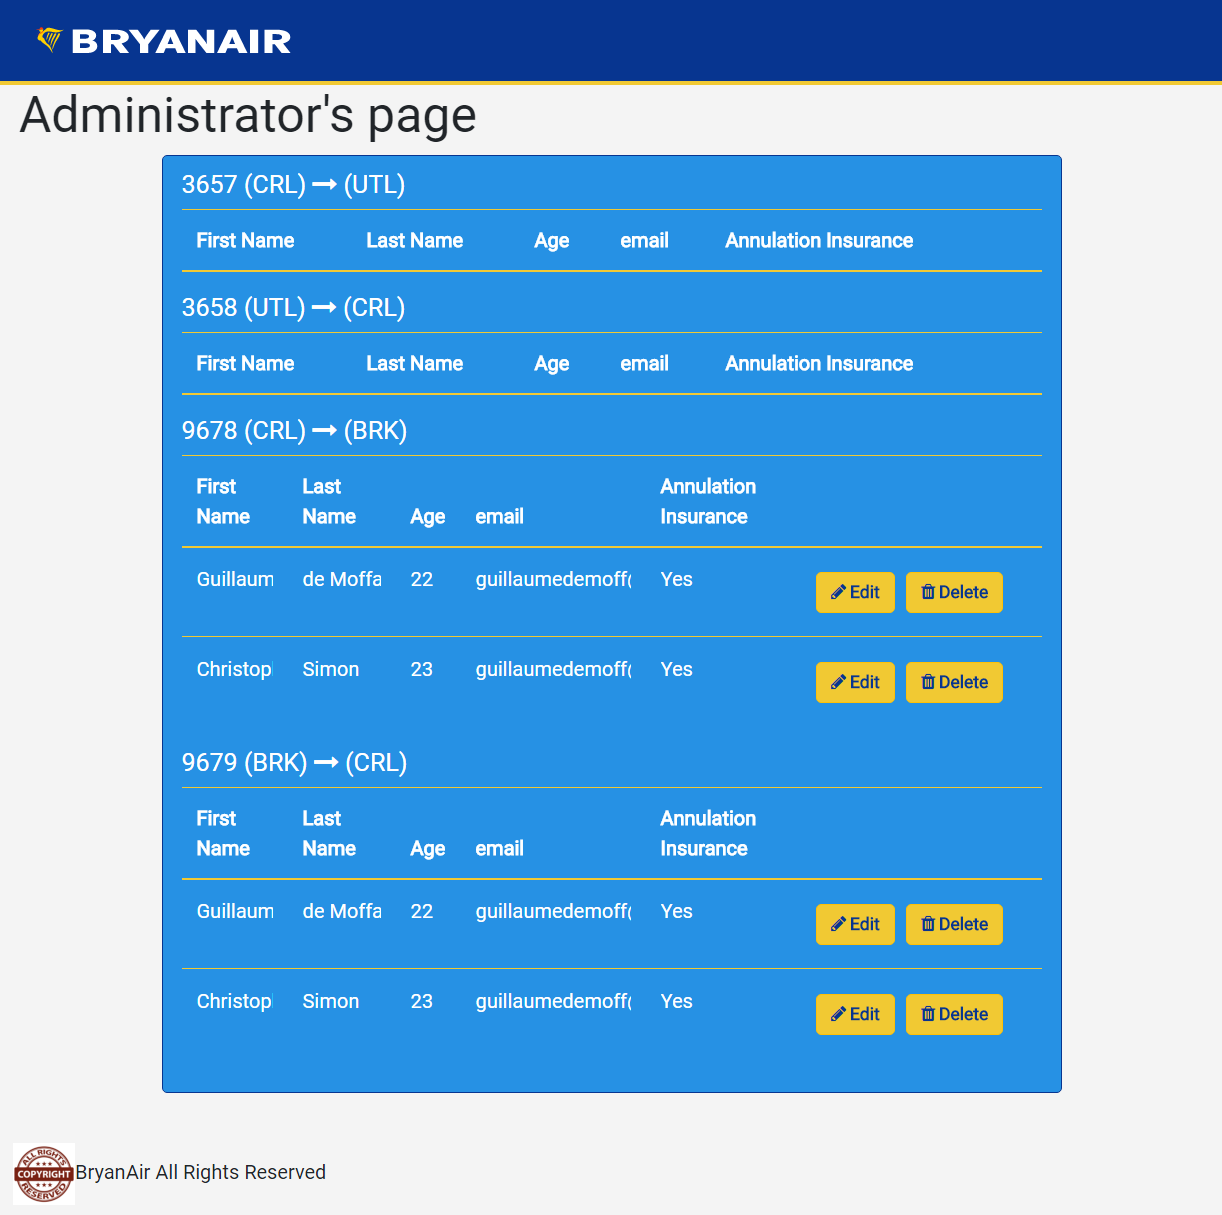
\includegraphics[width=\textwidth]{Admin.png}
			\caption{Page d'administration.}
			\label{fig:admin}
		\end{figure}

	\section{Fonctionnement}
		Cette section fournit les explications sur le fonctionnement des différentes parties de l'application, telles que le routage, les templates HTML, le fonctionnement des réservations et l'interface d'adminis\-tration.
		\subsection{Routage}
		L'application est basée sur le design pattern MVC. Nous avons donc un routeur, des modèles, des contrôleurs et des vues. Le routeur redirige les requêtes vers le contrôleur adéquat grâce à une variable HTTP \texttt{GET}. Ce contrôleur vérifie les informations venant des formulaires, les charge et les enregistre dans la base de données, et génère la page correspondante.

		L'accès à une page se fait via l'URL suivante \url{http://localhost/BryanAir/<nom_de_page>}. Elle est réécrite en \url{http://localhost/Bryanair?page=<nom_de_page>} pour que le routeur puisse rediriger vers le bon contrôleur. Nous avons fait ce choix pour que les différentes URLs soient plus simples. Cette réécriture se fait par Apache grâce à une configuration dans le fichier \texttt{.htaccess} (annexe~\ref{ann:other})et elle est mise en place grâce a des regex.

		\subsection{Templates}
		Pour faciliter la construction des vues, nous avons utilisé un sytème de templates HTML. Nous avons placé des balises de la forme \texttt{\$balise\$}, dans nos pages HTML, que le contrôleur remplace par des valeurs.

    La fonction \texttt{buildHTML} du fichier \texttt{utils.php} (annexe~\ref{ann:other}) construit d'abord la vue en concaté\-nant quatres fichiers HTML:
    \begin{itemize}
      \item Trois de ces fichiers sont communs à toutes les vues: \texttt{head.html}, \texttt{header.html} et \texttt{footer.html} (annexe~\ref{ann:tmp}).
      \item Le contenu propre spécifique de la vue est ajouté entre le header et le footer.
    \end{itemize}

		La fonction remplace ensuite chaque balise par une valeur (simple texte, bout d'HTML...) construite par le contrôleur. Pour cela, elle prend en paramètre une liste de paires clé/valeur, les clés correspondant aux balises et les valeurs contenant la chaine de caractères de remplacement.

		Cette méthode facilite la création des vues. En effet, il n'est plus nécessaire de copier dans tous les fichiers HTML des bouts de code communs. Cette méthode permet aussi de bien séparer la partie statique (HTML pur) des vues de la partie dynamique (en PHP) gérée par le contrôleur.

		\subsection{Réservation}
      Lorsque l'on effectue une réservation, le contrôleur dédié \texttt{controler\_reservation.php} (annexe~\ref{ann:ctr}) charge la liste de tous les aéroports présents dans la table \texttt{airport} de la base de données. Grâce à cette liste, il construit ensuite, comme expliqué à la section précédente, la vue initiale de la réservation.

			Lorsque l'utilisateur valide la première page de réservation (figure~\ref{fig:res1}), le contrôleur \linebreak[4] \texttt{controleur\_detail.php} vérifie tout d'abord certaines des valeurs transmises par la variable HTTP \texttt{POST}. Il faut donc bien vérifier que toutes les données transmises nécessaires au contrôleur ont bien été définies et que le type de chacune est correct. Par exemple, la variable contenant le nombre de passagers doit pouvoir être convertie en un entier. Il est important que cette vérification se fasse du coté serveur. En effet, si l'utilisateur passe bien par le formulaire, il ne devrait pas y avoir de problèmes. Mais une personne mal intentionnée peut tout à fait utiliser un outil tel que cURL pour envoyer n'importe quelle requête POST au serveur ou même changer l'HTML dans l'inspecteur du navigateur pour les contraintes des champs du formulaire.

      Si un problème survient dans la vérification des données, L'utilisateur reste sur le formulaire et reçoit un message d'erreur affiché en haut de celui-ci (figure~\ref{fig:error}). Sinon, le contrôleur cherche dans la base de données les numéros de vols (aller/retour) et le nombre de places restantes. S'il n'y a plus de place pour le vol aller ou retour, ou qu'il ne trouve pas de vol pour les aéroports sélectionnés,  un message d'erreur apparait également.


      Pour terminer, le contrôleur instancie un objet de type \texttt{Reservation} ainsi que deux objets \texttt{Flight} avec toutes les informations précédemment récoltées. Il construit ensuite la page HTML \texttt{detail.html} (annexe~\ref{ann:tmp}) permetant d'encoder les données passagers.

			\begin{figure}[!ht]
         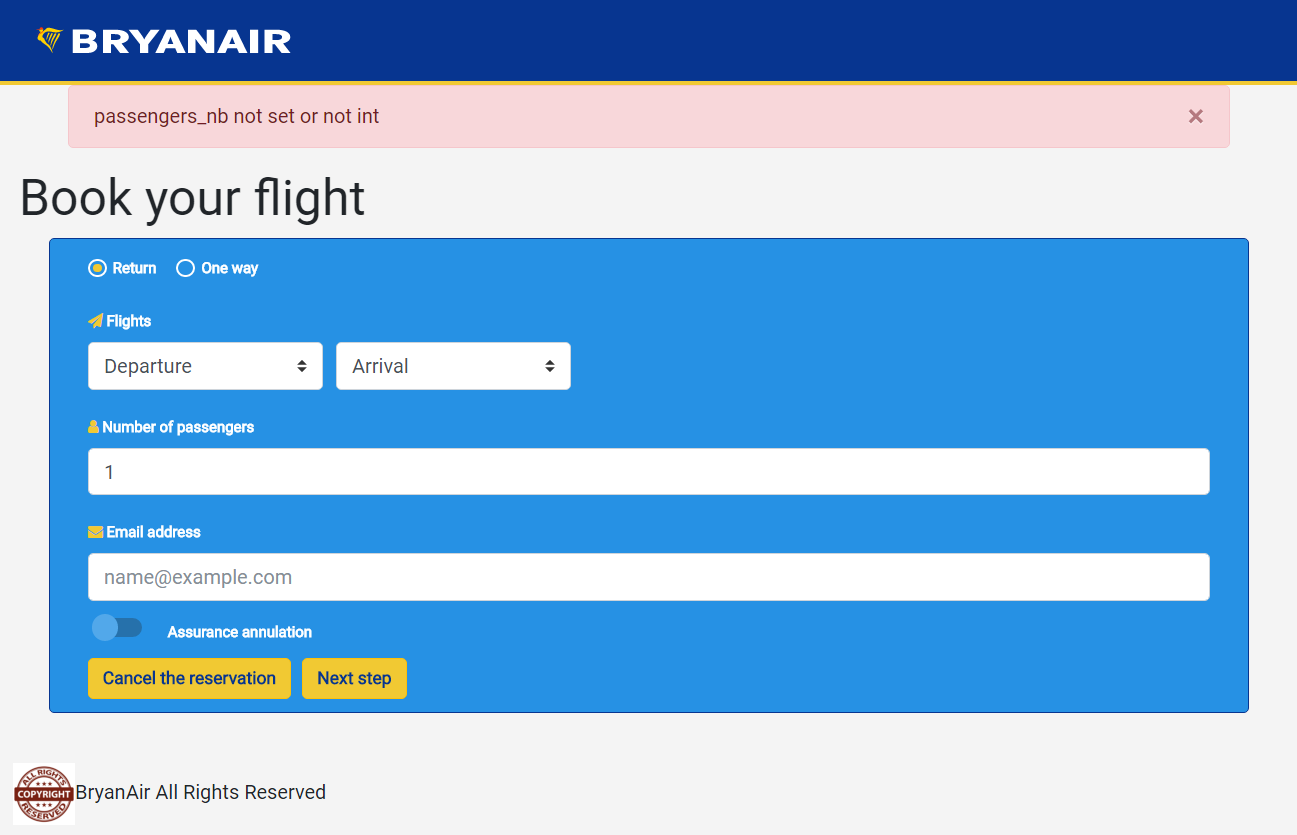
\includegraphics[width=\textwidth]{Error.png}
				\caption{Message d'erreur.}
				\label{fig:error}
			\end{figure}

			La deuxième étape de la réservation est celle où il faut encoder les informations des passagers, l'un après l'autre (figure~\ref{fig:res2}). Comme pour la première étape, celle-ci est gérée par un contrôleur dédié, \texttt{controleur\_nextpassenger.php} (annexe~\ref{ann:ctr}). Il commence par faire le même style de vérifications que précédement. Une fois la vérification passée, il instancie un objet de type \texttt{Client} qui est ajouté dans la liste de clients de l'objet \texttt{Reservation}. Le contrôleur reproduit la vue pour enregistrer un nouveau passager tant qu'il y en a. Une fois tous les passagers enregistrés, il construit la vue de confirmation \texttt{confirmation.html} (annexe~\ref{ann:tmp}).

			Une fois arrivé sur la page de confirmation, on a le choix entre confirmer la réservation ou l'annuler (figure~\ref{fig:conf}). Si la réservation est annulée, on est redirigé vers la page d'accueil et l'objet \texttt{Reservation} avec la liste des clients est supprimé. Si on confirme la réservation, le contrôleur \texttt{controler\_confirmation.php} (annexe~\ref{ann:ctr}) vérifie si au moins un des passagers est bien majeur. Si ce n'est pas le cas, le système d'erreur affiche un message (figure~\ref{fig:ageError}), et il faudra ré-encoder les informations de tous les passagers.

			\begin{figure}[!ht]
        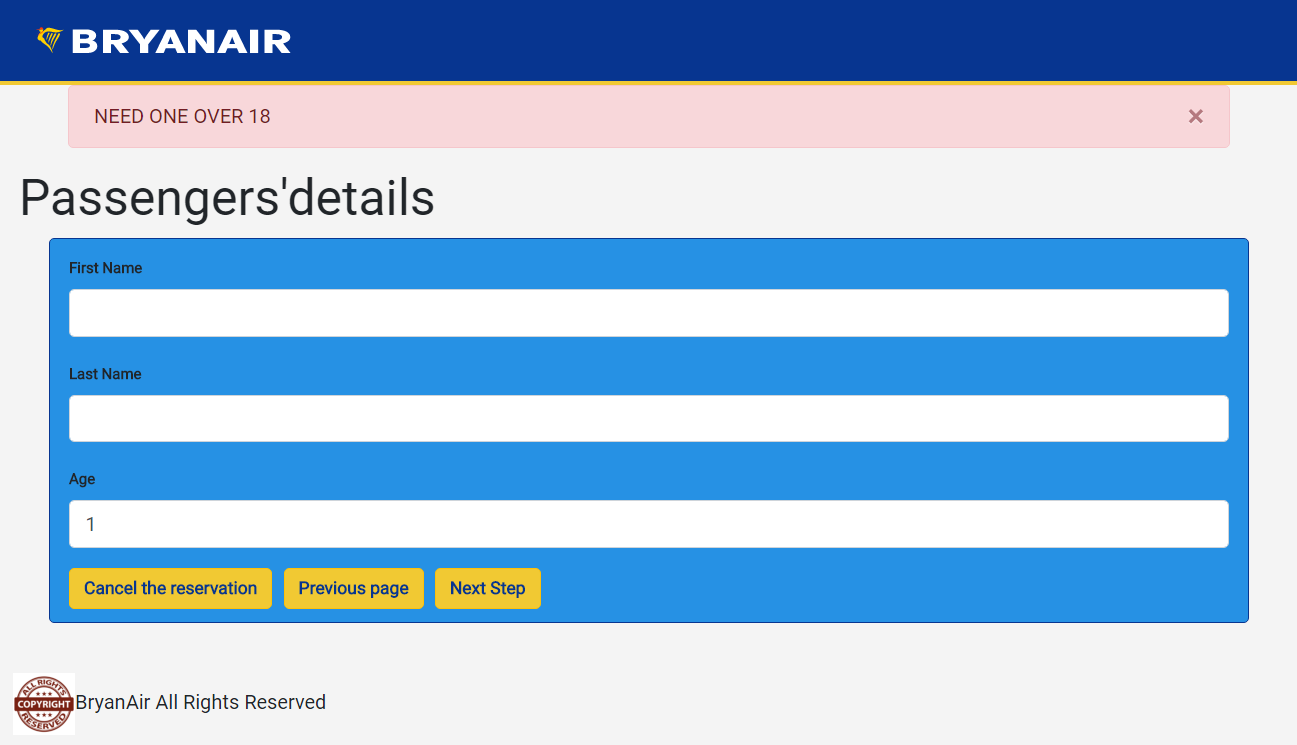
\includegraphics[width=\textwidth]{ageError.png}
				\caption{Erreur de majorité.}
				\label{fig:ageError}
			\end{figure}

			S'il y a bien au moins une personne majeure, le contrôleur enregistre les clients ainsi que leur réservation (une par client) dans la base de données et redirige vers une page résumant la réservation (figure~\ref{fig:recap}). Le contrôleur \texttt{controler\_resumer.php} (annexe~\ref{ann:ctr}) prend le relais et va tout d'abord construire un tableau HTML, avec tous les clients contenu dans la réservation. L'objet \texttt{Reservation} se charge aussi de calculer le prix total à payer en se basant sur le nombre de passagers, s'ils ont pris un vol aller-retour ou aller simple et enfin, si une assurance annulation à été prise. Un scénario détailé d'une réservation se trouve a l'annexe~\ref{ann:diag}.

		\subsection{Admin}
			La page admin est gérée par le contrôleur \texttt{controler\_admin.php} (annexe~\ref{ann:ctr}) qui charge depuis la base de données tous les vols ainsi que tous les passagers pour chacun d'entre eux. Il en fait un tableau HTML représentant toutes ces données puis construit la vue \texttt{admin.html} (annexe~\ref{ann:tmp}). Un scénario d'accès à l'espace admin se trouve a l'annexe~\ref{ann:diag}.

	\section*{Conclusion}
      Ce travail nous a apporté une meilleure connaissance du développement web, et plus particulière\-ment du modéle MVC, de la création d'une base de données Mysql et du développement PHP.

			Nous avons fait des efforts concernant le style de l'application en utilisant Bootstrap pour les différents boutons, les formulaires, les tableaux... et également défini le style de certains widgets depuis zéro (notamment le toggle). Des efforts ont également été apportés pour s'approcher le plus possible du site de Ryanair, comme le logo et l'icône, tous les deux réalisés au format vectoriel.

      Nous avons intégré une page error 404 personalisée pour les requêtes de pages qui n'existent pas sur BryanAir. Il y a également la possibilité de retourner sur la page d'accueil depuis n'importe quelle page en cliquant sur le logo présent dans le coin supérieur gauche de toutes les pages.

			Cependant, des améliorations sont possibles pour rendre l'application plus agréable à utiliser. Premièrement, ne pas devoir réencoder toutes les données des passagers en cas d'erreur. Pour terminer, nous aurions pu mettre le résumé de la réservation sur la page de confirmation pour que l'utilisateur ait les détails sous les yeux avant de confirmer.

\pagebreak
  \appendix
  \section{Modèles \label{ann:mdl}}
    \subsection{Client.php}
    \lstinputlisting[language=php]{\file{models/Client.php}}
    \subsection{Flight.php}
    \lstinputlisting[language=php]{\file{models/Flight.php}}
    \subsection{Reservation.php}
    \lstinputlisting[language=php]{\file{models/Reservation.php}}
\section{templates \label{ann:tmp}}
  \subsection{home.html}
  \lstinputlisting[language=html]{\file{templates/home.html}}
  \subsection{reservation.html}
  \lstinputlisting[language=html]{\file{templates/reservation.html}}
  \subsection{detail.html}
  \lstinputlisting[language=html]{\file{templates/detail.html}}
  \subsection{confirmation.html}
  \lstinputlisting[language=html]{\file{templates/confirmation.html}}
  \subsection{resumer.html}
  \lstinputlisting[language=html]{\file{templates/resumer.html}}
  \subsection{admin.html}
  \lstinputlisting[language=html]{\file{templates/admin.html}}
  \subsection{head.html}
  \lstinputlisting[language=html]{\file{templates/head.html}}
  \subsection{header.html}
  \lstinputlisting[language=html]{\file{templates/header.html}}
  \subsection{footer.html}
  \lstinputlisting[language=html]{\file{templates/footer.html}}
  \subsection{admin.html}
  \lstinputlisting[language=html]{\file{templates/admin.html}}

\section{Controlers \label{ann:ctr}}
  \subsection{controler\_home.php}
  \lstinputlisting[language=php]{\file{controler_home.php}}
  \subsection{controle\_reservation.php}
  \lstinputlisting[language=php]{\file{controler_reservation.php}}
  \subsection{controler\_detail.php}
  \lstinputlisting[language=php]{\file{controler_detail.php}}
  \subsection{controler\_nextpassenger.php}
  \lstinputlisting[language=php]{\file{controler_nextpassenger.php}}
  \subsection{controler\_confirmation.php}
  \lstinputlisting[language=php]{\file{controler_confirmation.php}}
  \subsection{controler\_resumer.php}
  \lstinputlisting[language=php]{\file{controler_resumer.php}}
  \subsection{controler\_admin.php}
  \lstinputlisting[language=php]{\file{controler_admin.php}}
  \subsection{controler\_update.php}
  \lstinputlisting[language=php]{\file{controler_update.php}}
  \subsection{controler\_delete.php}
  \lstinputlisting[language=php]{\file{controler_delete.php}}
  \subsection{controler\_404.php}
  \lstinputlisting[language=php]{\file{controler_404.php}}

\section{Other \label{ann:other}}
  \subsection{.htaccess}
  \lstinputlisting[language={}]{\file{.htaccess}}
  \subsection{index.php}
  \lstinputlisting[language=php]{\file{index.php}}
  \subsection{utils.php}
  \lstinputlisting[language=php]{\file{utils.php}}
  \subsection{style.css}
  \lstinputlisting[language=css]{\file{ressources/CSS/style.css}}

\section{Diagramme de séquence \label{ann:diag}}
  \subsection{Réservation}
  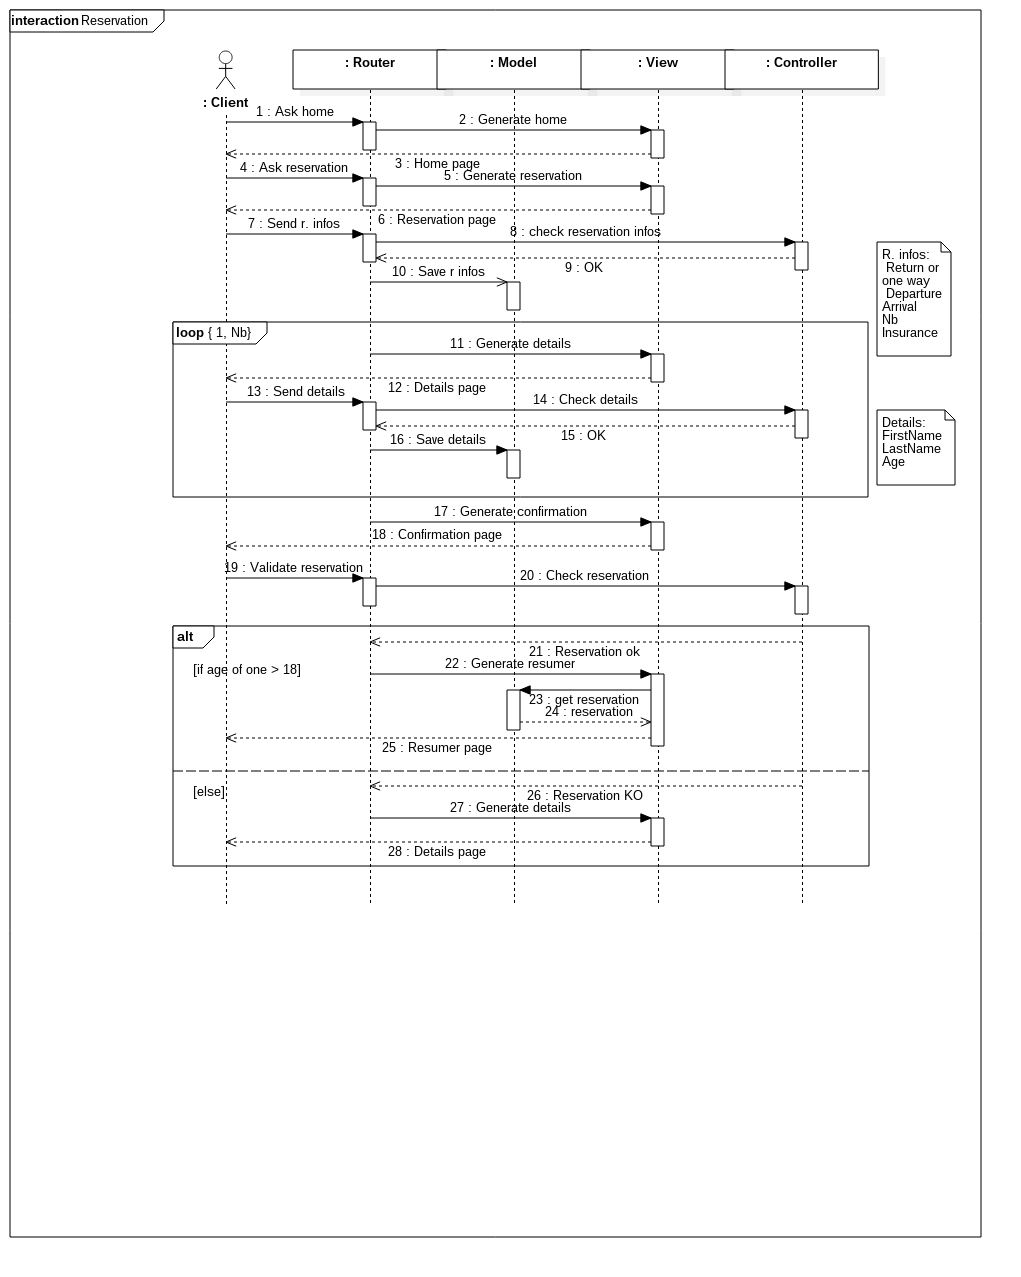
\includegraphics[width=\textwidth]{reservationDiagram}
  \subsection{Admin}
  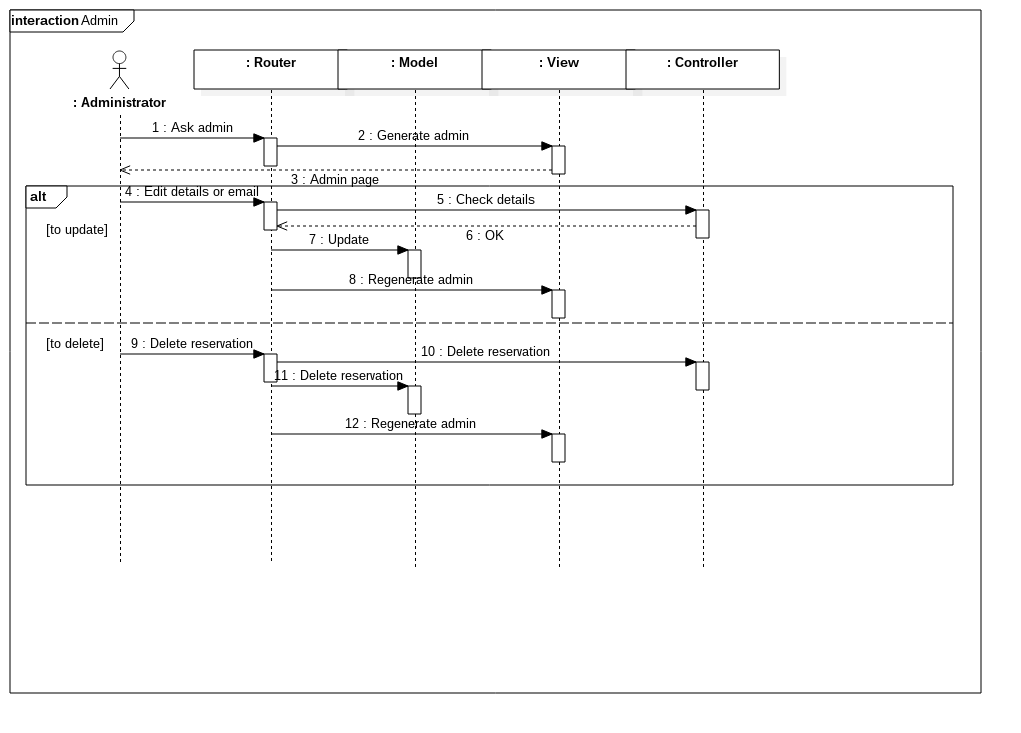
\includegraphics[width=\textwidth]{adminDiagram}
\end{document}
